%
% CHAPTER: Computational Creativity
%

\chapterimage{Wikipedia_Monument_2.pdf}

\chapter{Computational Creativity}
\label{chap:computational-creativity}

\begin{quote}
\begin{flushright}
\emph{To be surprised, to wonder, \\
is to begin to understand.}\\
José Ortega y Gasset \\
\end{flushright}
\end{quote}
\bigskip

In this Chapter we are going to see how to apply in practice our methodology for the assisted discovery of interesting research questions. As it was the case of previous chapter, in which we studied the concept of nescience from a practical point of view, ...

In the first part of this chapter we will see how to approximate the new metrics introduced: relevance and applicability. The relevance of a topic will be based on the number of web pages on Internet that link to the topic's page on Wikipedia (external links), and applicability will be estimated by the number of links from the Wikipedia's scientific pages to themselves (internal links). We will provide some practical examples of both quantities for the set of topics that compose the research area of theoretical computer science. Then, we will describe how to apply in practice our methodology for the discovery of interesting questions, and we will come up with some examples of new research questions that, in principle, could be addressed by science. The new questions proposed will be both, intradisciplinary, coming from the area of theoretical computer science, and interdisciplinary, by means of combining the area of theoretical computer science with the area of philosophy and the area of biochemistry. Finally, we will derive some new interesting research topics, according to our subjective interpretation of the combinations found, that are enough interesting to deserve to be the subject of new research activities. We will also evaluate if the proposed topics fulfill the requirements that we proposed in Chapter \ref{chap:Interesting-Research-Questions} for a question to be classified as interesting.

In the last part of the chapter, we will apply the set of metrics defined for the classification of individual research topics to full research areas. In this way, we will compute the interestingness of the different research disciplines as source of new problems, and their interestingness as a source of useful tools to solve open problems. These metrics will allow us to compare the relative merits of different knowledge disciplines. Some examples of research areas in decay will be shown as well.


\section{Interesting Research Questions}

Before to compute the new interesting questions, it is highly convenient to normalize the metrics of the topics involved in the study, otherwise, a very reduced set of topics could dominate all the questions. For the normalization process we have used the BoxCox method, that it is based on the identification of the best transformation from a family of power transformations.

{\color{red} TODO: Explain the BoxCox method} 

The most difficult part of the identification of topics as tools, that is, topics with very high maturity (or very low nescience), is to distinguish when the description of a topic is short because it is well understood (for example, a mathematical theorem), or when it is short because it is a unfinished or poorly written article. Our work is based on the classification of Wikipedia articles as stubs, however, this classification is not very reliable, since many stubs articles are not classified as such (many of the misclassified topics suffer from this problem). How to automatically distinguish between a well-understood topic and a poorly written description is still an open question.

By combining the elements of Table \ref{tab:Interestingness-of-Tools}
and Table \ref{tab:Interestingness-of-Problems} we could come up
with new interesting ideas of how to apply existing tools to open
problems. As it was said above, the goal of the approach described
in this article is to identify highly potential interesting applications,
but is up to the researcher to decide if certain combination of topics
make sense or not, and if they deserve the effort to pursuit them.
The results of the combination is in Table \ref{tab:Interesting-Intradisciplinary-Questions}.

\begin{table*}
\begin{centering}
\begin{tabular}{|l|c|c|}
\hline 
{Tool} & Problem & Interestingness\tabularnewline
\hline 
\hline 
Ternary numeral system & Regular expression & 1.21\tabularnewline
\hline 
{GNU MPAL} & Arithmetical hierarchy & 1.19\tabularnewline
\hline 
IEEE 854-1987 & Arithmetical hierarchy & 1.17\tabularnewline
\hline 
Quantum computer & Regular expression & 1.17\tabularnewline
\hline 
Ternary numeral system & Arithmetical hierarchy & 1.15\tabularnewline
\hline 
Division by zero & Regular expression & 1.15\tabularnewline
\hline 
Turing machine & Regular expression & 1.14\tabularnewline
\hline 
GNU MPAL & Regular expression & 1.13\tabularnewline
\hline 
Ternary numeral system & Halting problem & 1.13\tabularnewline
\hline 
Recursion & Halting\_problem & 1.13\tabularnewline
\hline 
\end{tabular}
\par\end{centering}

\caption{\label{tab:Interesting-Intradisciplinary-Questions}Interesting Intradisciplinary
Questions}
\end{table*}

Most of the interesting questions identified have very low quality.
As it was said before, the problem is that it is very difficult to
distinguish (automatically and unsupervised) between a poorly written
article from a very well understood topic. In this section we review
some on the interesting intradisciplinary questions identified with
the aim to clarify what we mean as interesting question and how interesting
questions should be interpreted. Some combinations worth examining
could be:
\begin{itemize}
\item Interesting Question 7: \emph{Can we apply }Turing machines\emph{
to }regular expressions\emph{?} The answer to this question is yes,
since it is a very well know question. Regular expressions are recognized
by finite automata, and finite automata can be simulated by Turing
machines.
\item Interesting Question 10: \emph{Can we apply }recursion\emph{ to the
}halting problem\emph{?} Again the answer is yes, since the proof
of the halting problem is based on a machine that call itself.
\end{itemize}
Note that both questions have well known answers, and so, we have
failed to provide original questions.

The most interesting questions arise when we combine topics from two
different disciplines. However, the probability that the identified
questions are meaningful is lower than in the case of intradisciplinary
analysis.

For the interdisciplinary analysis we have used the collection of
pages from the theory of computation already used in the intradisciplinary
analysis, and a new collection of topics from the area of\emph{ }bioinformatics.
The topics were selected using the Wikipedia category \emph{natural
sciences}, \emph{biology}, \emph{bio}logical\emph{ processes}. In
total, there were more than $10^{5}$ combinations analyzed. Table
\ref{tab:Interesting-Intradisciplinary-Questions-1-1} contains the
list of the most relevant intradisciplinary applications.

\begin{table*}
\begin{centering}
\begin{tabular}{|l|c|c|}
\hline 
{Tool} & Problem & Interestingness\tabularnewline
\hline 
\hline 
State space & Action potential & 1.17\tabularnewline
\hline 
{Turing machine} & Action potential & 1.16\tabularnewline
\hline 
Quantum computer & Action potential & 1.16\tabularnewline
\hline 
Abstract machine & Action potential & 1.14\tabularnewline
\hline 
Computational model & Action potential & 1.13\tabularnewline
\hline 
State space & Membrane potential & 1.12\tabularnewline
\hline 
State space & Meiosis & 1.11\tabularnewline
\hline 
Arithmetic logic unit & Meiosis & 1.11\tabularnewline
\hline 
GNU MPAL & Flashbulb memory & 1.11\tabularnewline
\hline 
Ternary numeral system & Working memory & 1.10\tabularnewline
\hline 
\end{tabular}
\par\end{centering}

\caption{\label{tab:Interesting-Intradisciplinary-Questions-1-1}Interesting
Interdisciplinary Questions}
\end{table*}

The set of interdisciplinary questions also suffer from the problem
of the stub articles, and so, the quality of the results is low. Some
interdisciplinary applications could be:
\begin{itemize}
\item Interesting question 1: \emph{Can we apply state space to action potential?}
Questions 1, 2, 3, 4 and 5, all of them, suggest the same idea, that
is, if it is possible to formalize the concept of action potential,
in such a way that can be reproduced by a computer.
\item Interesting question 7: \emph{Can we apply state space to meiosis?}
Question 7 is similar to question 1, and it asks about the possibility
of formalize the concept of meiosis using a computer.
\end{itemize}

\subsection{Relevance}

In Definition \ref{def:relevance} we introduced the concept of relevance of a research topic as a measure of the impact that this topic could have in people's life. The idea was that the higher the relevance, the higher its potential as a source of interesting questions, since we would be addressing a problem that affects many people. Relevance was defined as the degree of the research topic in the relevance graph, a bipartite graph connecting topics and people (see Definition \ref{def:relevance-graph}). Of course, this relevance graph is a mathematical abstraction that it is very difficult to compute in practice, since we do not have information about how people is affected by each topic.

As an approximation of the relevance of a topic we have used the number of links (URLs) from external web pages on the whole Internet that point to the topic's web page on Wikipedia. The rationale is that the more relevant is a topic, the more people will be talking about it on Internet, and the more URLs there will be linking to Wikipedia, since Wikipedia is a well known source of information to which many people refer. In fact, we are not interested in knowing the absolute relevance of research topics, since what we need is a measure of relative relevance between different topics. An underestimate of the relevance is not harmful as long this underestimation is equally distributed among all the topics. It requires further research to fully understand how well the the theoretical concept of relevance is approximated by this URLs counting procedure. 

Another problem is that we do not know the number of links to a web page on Internet, and so, we have to apply a second approximation. In this case, the number of links was estimated using Google's \texttt{link:} facility in searches. Google's \texttt{link:} lists the links that Googlebot discovered during its crawling and indexing process of Internet. For example, the number of external pages that link to the \emph{Computer Science} article in Wikipedia is given by:

\smallskip

\texttt{
link:http://en.wikipedia.org/wiki/Computer\_science
}

\smallskip

As Google recognizes in its web page, not all links to a site may be listed. The number of links could vary due to redirections, crawling errors, and other problems. How these errors affect to the accuracy of the links counting is not clear, since the details of the Google's crawling algorithm are not public.

Figure \ref{fig:Relevance-of-Topics} shows a plot of the relevance of the set of topics after the application of the normalization process described in {\color{red} XXX}. A practical problem is that there are too many topics with a very low number of links (as indexed by Google). That should not be a problem since we are not using at any moment those topics with very low relevance.

\begin{figure}[h]
\centering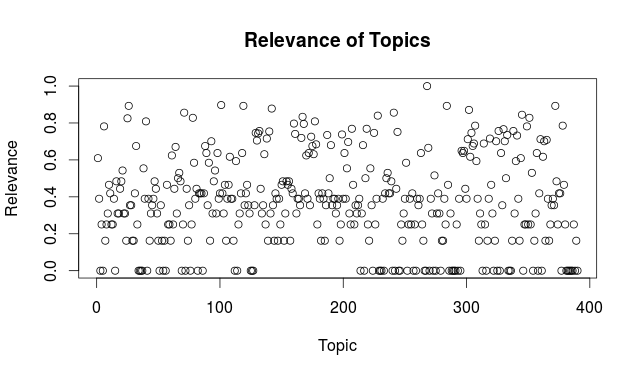
\includegraphics[scale=0.5]{RelevanceTopics}
\caption{\label{fig:Relevance-of-Topics}Relevance of topics}
\end{figure}

Table \ref{tab:Relevance-of-Topics} contains the ten most relevant topics according to its relevance. For each topic it is shown it relevance (number or external links) and the normalized version of this number. The list includes basic concepts (\emph{binary number,} \emph{floating point}), advanced concepts (\emph{Turing machine}, \emph{finite-state machine, cellular automaton, lambda calculus}, \emph{Turing completeness}), highly popular tools (\emph{recursion}, \emph{regular expression}) and classical problems (\emph{halting problem}). All those topics could fit into our intuitive idea of highly relevant, although some authors could perfectly disagree that some of them are the most relevant ones in the area of theory of computation (for example, \emph{floating point}).

\begin{table}
\begin{centering}
\begin{tabular}{|c|c|c|}
\hline 
Topic & Relevance & Norm.\tabularnewline
\hline 
\hline 
Regular expression & 409 & 1.00\tabularnewline
\hline 
Turing machine & 159 & 0.90\tabularnewline
\hline 
Binary number & 141 & 0.89\tabularnewline
\hline 
Recursion & 133 & 0.88\tabularnewline
\hline 
Finite-state machine & 118 & 0.86\tabularnewline
\hline 
Halting problem & 108 & 0.85\tabularnewline
\hline 
Cellular automaton & 104 & 0.85\tabularnewline
\hline 
Floating point & 99 & 0.84\tabularnewline
\hline 
Lambda calculus & 95 & 0.84\tabularnewline
\hline 
Turing completeness & 93 & 0.83\tabularnewline
\hline 
\end{tabular}
\par\end{centering}

\caption{\label{tab:Relevance-of-Topics}Relevance of topics}
\end{table}

\subsection{Applicability}

Applicability measures how likely is that a research topic can be applied to solve open problems. If a tool has been already applied to solve multiple problems, then there is a high probability that it can be used again to solve new problems. The number of problems in which a tool has been applied is computed with the aid of the applicability graph (see Definiton \ref{def:applicability-graph}), and applicability is formally defined as the out-degree of the topic in this graph (see Definiton \ref{def:applicability}). We have approximated the applicability graph by means of using the graph of internal links between the scientific pages of Wikpiedia. That is, we approximate the applicability of a topic by counting the number of pages from Wikipedia domain that links to the topic's page (we have used the \emph{``What links here''} facility from Wikipedia, a tool to see the list of the pages that link to, or redirect to, the current page). As it was the case of the relevance of a topic, we are not intersted in the absolute value of the applicability of topics. What it is important for us is the relative ordering of topics based on their applicability. Perhaps, a better approach to approximate the applicability of a topic would be to analyze the graph of citations from academic research papers, combined with the automatic identification of the topics addressed in those papers.

% TODO: Perhaps we could include a nice picture of the graph of Wikipedia internal links

The applicability of a topic Figure \ref{fig:Applicability-of-Topics} shows a plot of the applicability of the selected set of topics after the normalization process, and Table \ref{tab:Applicability-of-Topics} contains the ten most relevant topics according to its applicability. For each topic it is shown the number or internal links and the normalized version of this number. In the list we can find topics like \emph{regular expression}, \emph{recursion}, \emph{Turing machine}, or \emph{cellular automaton} that perfectly fits our intuitive idea of tools that can be applied to solve other problems. However, we can also find in the list the topic \emph{quantum computer} that is not very applicable, but since it is a highly popular research topic it is mentioned in many different Wikipedia's pages. Other pages like \emph{division by zero}, \emph{floating point}, or \emph{binary number}, do not seems to be good tools either. The final topic, \emph{computatibility theory}, shows that, even at the fourth level, we still can find too broad topics.

\begin{figure}[h]
\centering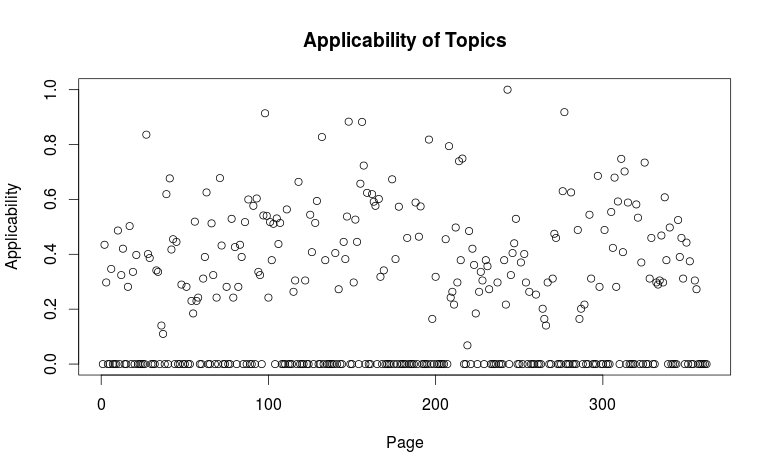
\includegraphics[scale=0.5]{ApplicabilityTopics}
\caption{\label{fig:Applicability-of-Topics}Applicability of topics}
\end{figure}

\begin{table}
\begin{centering}
\begin{tabular}{|c|c|c|}
\hline 
Topic & Applicab. & Norm.\tabularnewline
\hline 
\hline 
Regular expression & 1971 & 1.00\tabularnewline
\hline 
Recursion & 1227 & 0.91\tabularnewline
\hline 
Quantum computer & 1197 & 0.91\tabularnewline
\hline 
Division by zero & 998 & 0.88\tabularnewline
\hline 
Floating point & 992 & 0.88\tabularnewline
\hline 
Turing machine & 748 & 0.83\tabularnewline
\hline 
Binary number & 710 & 0.82\tabularnewline
\hline 
Ternary num. sys. & 670 & 0.80\tabularnewline
\hline 
Cellular automaton & 433 & 0.74\tabularnewline
\hline 
Computability theory & 430 & 0.73\tabularnewline
\hline 
\end{tabular}
\par\end{centering}

\caption{\label{tab:Applicability-of-Topics}Applicability of topics}
\end{table}


\subsection{Intradisciplinary Questions}

The interest of a topic as a tool measures how likely is that this
tool can be applied to other problems. Figure \ref{fig:Interestingness-of-Tools}
shows a plot of the interestingness of the selected set of topics
after the normalization process.

\begin{figure}[h]
\centering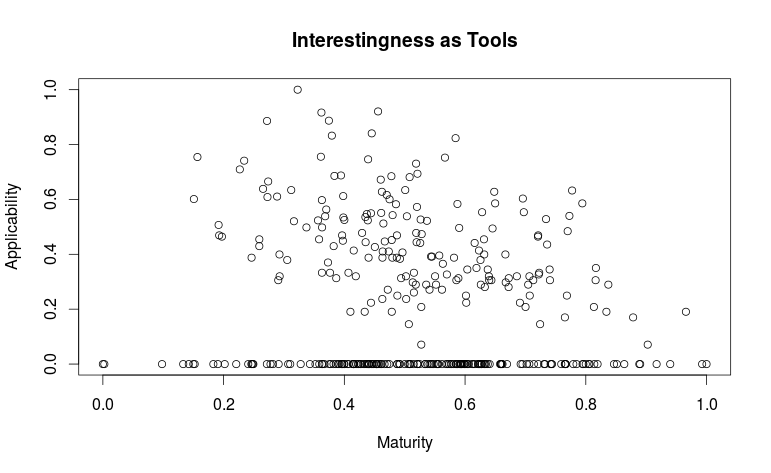
\includegraphics[scale=0.5]{InterestingnessTools}
\caption{\label{fig:Interestingness-of-Tools}Interestingness of Tools}
\end{figure}

Table \ref{tab:Interestingness-of-Tools} contains the ten most relevant
topics according to its interestingness as a source of interesting
tools. Out of the ten topics, only two (\emph{ternary numeral system}
and \emph{recursion}) appear in the list of top ten mature topics
or top ten applicable topics; the rest of topics are new. In the list
we can find topics like the \emph{GNU Multiple Precision Arithmetic
Library} and the \emph{standard for radix-independent floating-point
arithmetic} (IEEE 854-1987) that are definitely tools, but not in
the sense of tool that we are looking for our methodology. Some other
topics are not clear that can be considered as tools, like \emph{arithmetic
logic unit}, \emph{barrel shifter}, or \emph{arithmetic overflow}.
Topics that match or intuitive idea of tool include \emph{recursion},
\emph{state space}, \emph{abstract machine}, and \emph{ternary numeral
system}. There are also some topics, like \emph{computational model},
too broad to be considered in a question.

\begin{table}
\begin{centering}
\begin{tabular}{|c|c|}
\hline 
Topic & Interestingness\tabularnewline
\hline 
\hline 
GNU MPAL & 0.49\tabularnewline
\hline 
Ternary numeral system & 0.48\tabularnewline
\hline 
IEEE 854-1987 & 0.47\tabularnewline
\hline 
Arithmetic logic unit & 0.43\tabularnewline
\hline 
Recursion & 0.42\tabularnewline
\hline 
Barrel shifter & 0.42\tabularnewline
\hline 
State space & 0.42\tabularnewline
\hline 
Abstract machine & 0.41\tabularnewline
\hline 
Computational model & 0.39\tabularnewline
\hline 
Arithmetic overflow & 0.39\tabularnewline
\hline 
\end{tabular}
\par\end{centering}

\caption{\label{tab:Interestingness-of-Tools}Interestingness of Tools}
\end{table}

Finally, Figure \ref{fig:Interestingness-of-Questions} contains a
plot of the interestingness of the topics considered as potential
interesting problems.

\begin{figure}[h]
\centering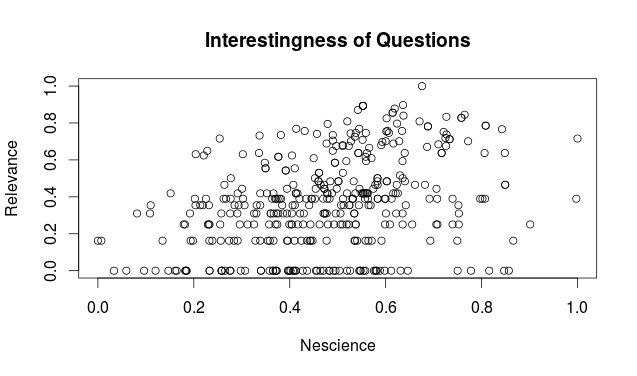
\includegraphics[scale=0.5]{InterestingnessQuestions}
\caption{\label{fig:Interestingness-of-Questions}Interestingness of Questions}
\end{figure}

Table \ref{tab:Interestingness-of-Problems} shows the ten most interesting
topics as interesting problems. Topics that fit our intuitive idea
of problem, that is, not very well understood concepts with a high
relevance, could include \emph{arithmetical theory}, \emph{halting
problem}, \emph{floating point}, \emph{quantum computer}, and \emph{computable
function}. The topic \emph{recursion} appears both as a tool and as
a problem. However in case of tools it refers to the concept of recursion
in general, and in case of problems it refers to the implementation
of the concept of recursion in the particular case of computer science.
The case of \emph{regular expression}, a topic that intuitively should
be classified as a tool and not as a problem, can be explained due
to the length of the article in Wikipedia, that provides a detailed
description of the language used for regular expressions. This problem
rises the question of how to distinguish in Wikipedia between introductory
articles and reference articles. Finally, there are topics like \emph{computability
theory}, \emph{lambda calculus} and \emph{computability} that are
too broad to be analyzed as problems.

\begin{table}
\begin{centering}
\begin{tabular}{|c|c|}
\hline 
Topic & Interestingness\tabularnewline
\hline 
\hline 
Arithmetical hierarchy & 0.72\tabularnewline
\hline 
Regular expression & 0.68\tabularnewline
\hline 
Computability theory & 0.65\tabularnewline
\hline 
Halting problem & 0.65\tabularnewline
\hline 
Recursion (CS) & 0.64\tabularnewline
\hline 
Lambda calculus & 0.63\tabularnewline
\hline 
Floating point & 0.61\tabularnewline
\hline 
Quantum computer & 0.57\tabularnewline
\hline 
Computability & 0.55\tabularnewline
\hline 
Computable function & 0.55\tabularnewline
\hline 
\end{tabular}
\par\end{centering}

\caption{\label{tab:Interestingness-of-Problems}Interestingness of Problems}
\end{table}

\begin{remark}
Based on the given definition of "Interestingness of a topic as a tool", we can explore various mathematical properties and concepts derived from this idea. Some possibilities include:

\begin{itemize}

\item Normalization: To compare different topics fairly, we can normalize their interestingness values by scaling them to a specific range, e.g., [0, 1]. This normalization can help compare the relative interestingness of various topics.

\item Weighted Interestingness: We can introduce weights to the maturity and applicability dimensions to emphasize one over the other depending on the specific context or application. This would allow us to fine-tune the interestingness measure for different scenarios.

\item Correlation: Studying the correlation between maturity and applicability could provide insights into how these dimensions are related and possibly reveal trends across different research topics.

\item Cluster Analysis: By examining topics in the two-dimensional vector space defined by maturity and applicability, we can perform cluster analysis to identify groups of topics with similar levels of interestingness. This can help identify areas of research that share characteristics and possibly suggest interdisciplinary research opportunities.

\item Rate of Change: Investigating the rate of change of interestingness over time can provide insights into the evolving landscape of a research field. This analysis could reveal emerging topics or those that are becoming less relevant.

\item Optimization: Using the interestingness metric, we can explore optimization techniques to find the most interesting topics given certain constraints or within specific domains. This could be useful for research prioritization and resource allocation.

\end{itemize}

These derived mathematical properties and concepts can provide a deeper understanding of the interestingness of research topics and their potential application as tools for solving problems.

\end{remark}



\subsection{Interdisciplinary Questions}

\section{New Research Topics}

If we combine the list of highly relevant and not very well understood
problems with themselves, it might happen that we come up with a new
topic that lies in the new unknown unknown area.

In Figure \ref{fig:Interesting-Intradisciplinary-Qu} it is shown
a plot%
\footnote{With the aim to make the figure clear, only a reduced set of the topics
is depicted.%
} of the interestingness of the (potential) new topics compared with
the interestingness of the topics that generated them.

\begin{figure}[h]
\centering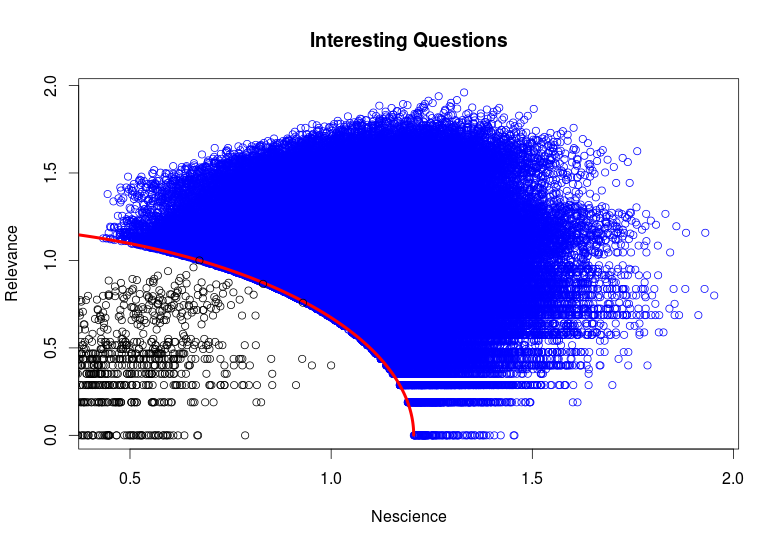
\includegraphics[scale=0.5]{NewQuestions}
\caption{\label{fig:Interesting-Intradisciplinary-Qu}Interesting Intradisciplinary
Questions}
\end{figure}

Table \ref{tab:Serendipity-Topics} contains a list of the top 25
candidates to become new topics topics according to their interestingness.
In this analysis we have included all the topics from all the knowledge
areas. Most of the questions deal with the concept of intellectual
property (\emph{copyright}, \emph{open access}, \emph{public domain},
and perhaps, \emph{wiki}), suggesting that this is an area where there
are still a lot of things to discover, much more that we are aware
of. Perhaps, it could be also a problem of a certain bias of Wikipedia
to these, and related, topics. Further investigation is required to
clarify this point.

In order to understand how new topics are generated, we have selected
the following two examples:
\begin{itemize}
\item New topic 17: \emph{Public domain + Earth}. This question rises the
issue if the Earth should be considered as a public resource; it touches
the very concept of private property. The methodology suggest that
this is not a very well understood topic.
\item New topic 18: \emph{Public domain + Internet}. Raises the same issue
that Question 17, but in this case restricted to Internet and its
governance.
\end{itemize}
Unfortunately, in both cases we fail to provide a well defined, innovative,
and previously unseen, research topic.

\begin{table*}
\begin{centering}
\begin{tabular}{|l|c|c|}
\hline 
{Problem} & Problem & Interestingness\tabularnewline
\hline 
\hline 
Public domain & Open access & 1.71\tabularnewline
\hline 
{Public domain} & REST & 1.70\tabularnewline
\hline 
Public domain & Wiki & 1.70\tabularnewline
\hline 
Open access & REST & 1.70\tabularnewline
\hline 
Copyright & Public domain & 1.69\tabularnewline
\hline 
Open access & Wiki & 1.69\tabularnewline
\hline 
Public domain & QR code & 1.69\tabularnewline
\hline 
Copyright & Open access & 1.68\tabularnewline
\hline 
Wiki & REST & 1.68\tabularnewline
\hline 
Open access & QR code & 1.68\tabularnewline
\hline 
Public domain & Transport Layer Security & 1.68\tabularnewline
\hline 
Copyright & REST & 1.68\tabularnewline
\hline 
QR code & REST & 1.67\tabularnewline
\hline 
Open access & Transport Layer Security & 1.67\tabularnewline
\hline 
Copyright & Wiki & 1.67\tabularnewline
\hline 
Wiki & QR code & 1.67\tabularnewline
\hline 
Public domain & Earth & 1.67\tabularnewline
\hline 
Public domain & Internet & 1.67\tabularnewline
\hline 
REST & Transport Layer Security & 1.66\tabularnewline
\hline 
Copyright & QR code & 1.66\tabularnewline
\hline 
Earth & Open access & 1.66\tabularnewline
\hline 
Internet & Open access & 1.66\tabularnewline
\hline 
Public domain & Open source & 1.66\tabularnewline
\hline 
Public domain & Web 2.0 & 1.66\tabularnewline
\hline 
Wiki & Transport Layer Security & 1.66\tabularnewline
\hline 
\end{tabular}
\par\end{centering}

\caption{\label{tab:Serendipity-Topics}New Topics}
\end{table*}


We could also restrict our search of new topics to a reduced number
of knowledge categories. For example, in Table \ref{tab:Restricted-Serendipity}
contains the ten most interesting new topics corresponding to the
already studied areas of \emph{theory of computation} and a new area
of \emph{phenomenology} (from Level 2 \emph{philosophy of mind}, and
Level 1 \emph{cognitive science}). Given the list of topics contained
in the table, we could come up with, for example, the following potential
new topics:
\begin{itemize}
\item New topic 2:\emph{ Turing machine} + \emph{synesthesia}: this new
topic could be about a new kind of Turing machine that incorporates
synesthesic properties. These new s\emph{ynesthesic Turing machines}
could be defined as the union of a group of Turing machines that are
linked together in such a way that when one machines read a symbol
from its tape, it produces an automatic change in the state of another
machine. The property of synesthesia could be also extended to the
case of non-deterministic Turing machines.
\item New topic 4:\emph{ Kolmogorov Complexity} + \emph{Self-awarenes}:
This topic could be interpreted as investigating the minimum complexity
required for a computer program to have the capacity of self-awareness.
\end{itemize}
\begin{table*}
\begin{centering}
\begin{tabular}{|l|c|c|}
\hline 
{Question} & Question & Interestingness\tabularnewline
\hline 
\hline 
Kolmogorov complexity & Change blindness & 1.24\tabularnewline
\hline 
{Turing machine} & Synesthesia & 1.23\tabularnewline
\hline 
Kolmogorov complexity & Qualia & 1.23\tabularnewline
\hline 
Kolmogorov complexity & Self-awareness & 1.22\tabularnewline
\hline 
Turing machine & Qualia & 1.22\tabularnewline
\hline 
Kolmogorov complexity & Synesthesia & 1.21\tabularnewline
\hline 
Turing completeness & Synesthesia & 1.20\tabularnewline
\hline 
Turing machine & Self-awareness & 1.20\tabularnewline
\hline 
Turing completeness & Qualia & 1.20\tabularnewline
\hline 
Turing completeness & Self-awareness & 1.18\tabularnewline
\hline 
\end{tabular}
\par\end{centering}

\caption{\label{tab:Restricted-Serendipity}Restricted New Topics}
\end{table*}


\section{References}

Papers about the BoxCox method ...

\section{Future Work}


